\documentclass{article}
\usepackage[letterpaper, margin=0.3in]{geometry}
\usepackage{multicol}
\usepackage{graphicx}
\usepackage{amsmath}

\begin{document}
\LARGE
\section{Quotient Identities}
\hrule
\begin{multicols}{3}
    \noindent
    $\sin \theta = \dfrac{O}{H}$                       \\\\
    $\sin \theta = \cos \theta \tan \theta$\\\\
    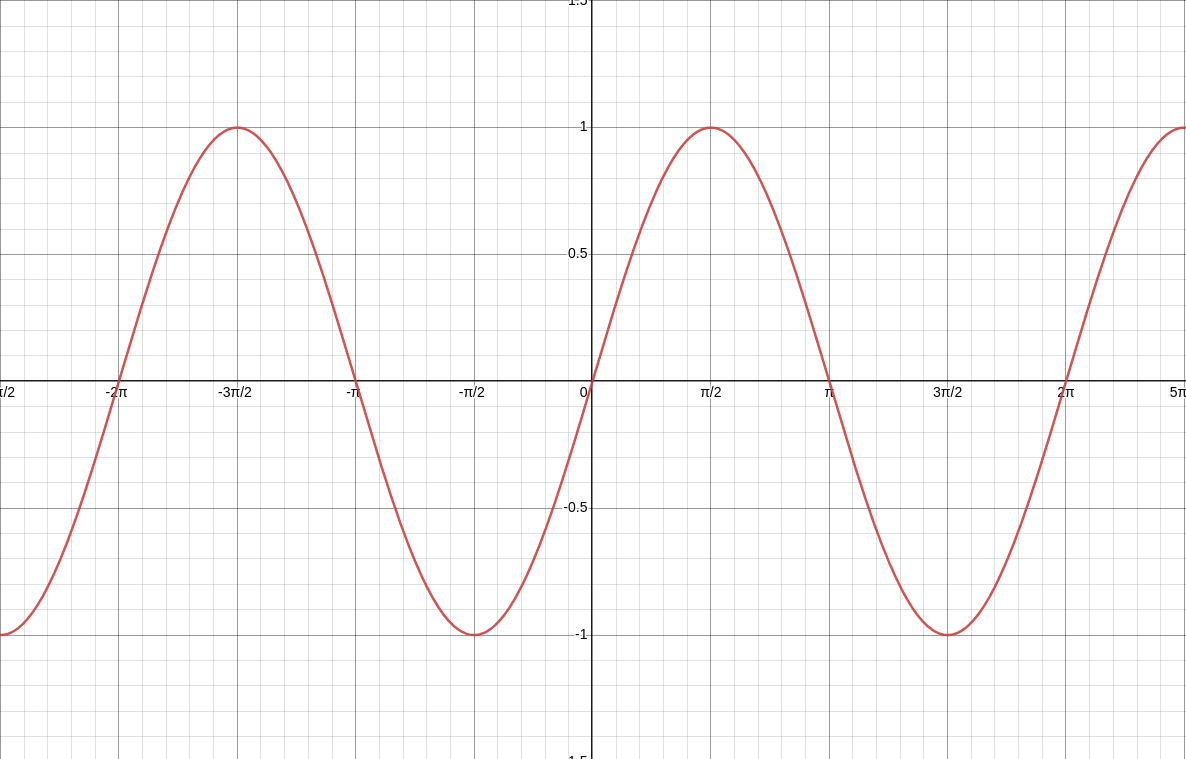
\includegraphics[scale=0.15]{images/sin.png}       \\
    $\cos \theta = \dfrac{A}{H}$                       \\\\
    $\cos \theta = \dfrac{\sin \theta}{\tan \theta}$   \\\\
    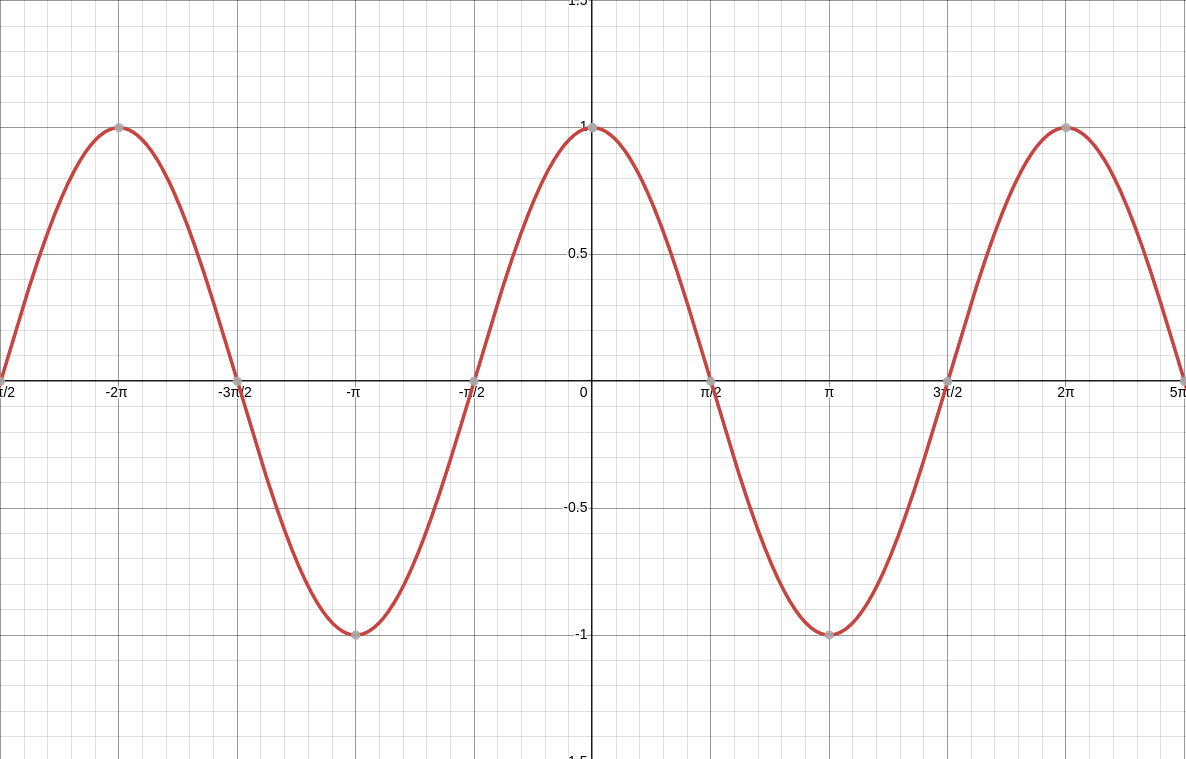
\includegraphics[scale=0.15]{images/cos.png}       \\
    $\tan \theta = \dfrac{O}{A}$                       \\\\
    $\tan \theta = \dfrac{\sin \theta}{\cos \theta}$   \\\\
    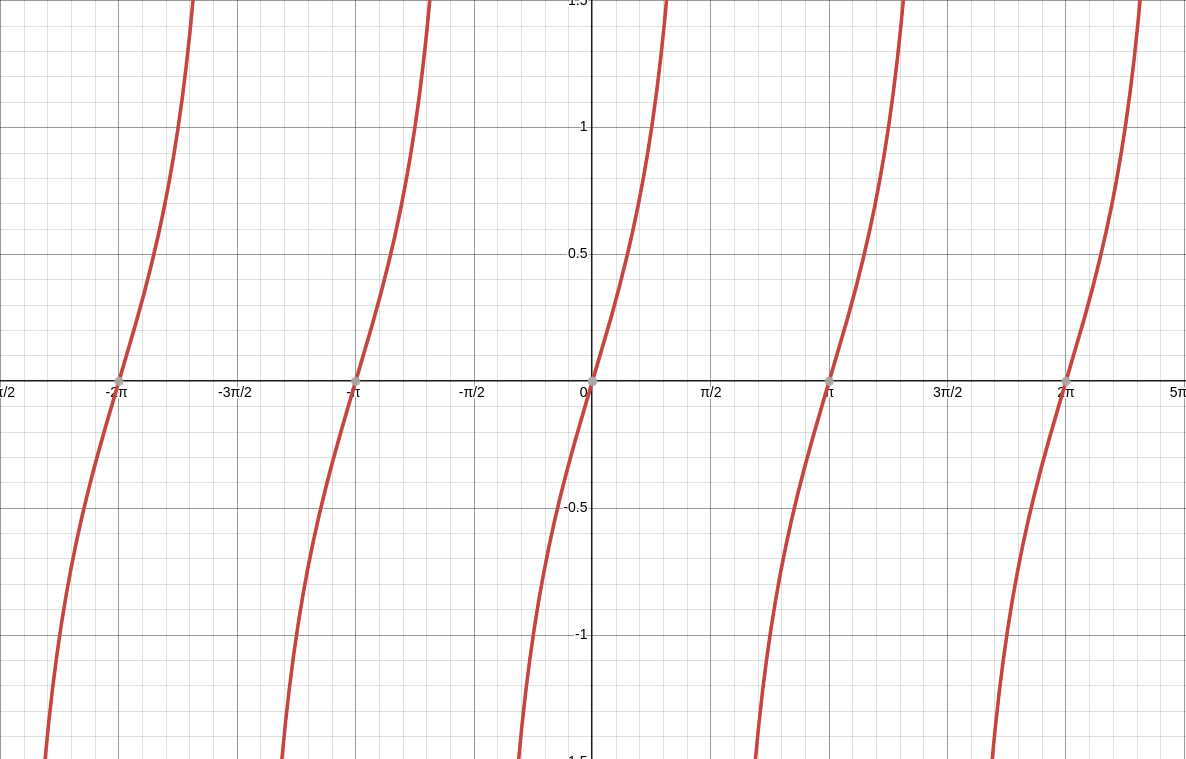
\includegraphics[scale=0.15]{images/tan.png}
\end{multicols}
\section{Reciprocal Identites}
\hrule
\begin{multicols}{3}
    \noindent
    $\csc \theta = \dfrac{1}{\sin \theta}$        \\\\
    $\csc \theta = \dfrac{H}{O}$                  \\\\
    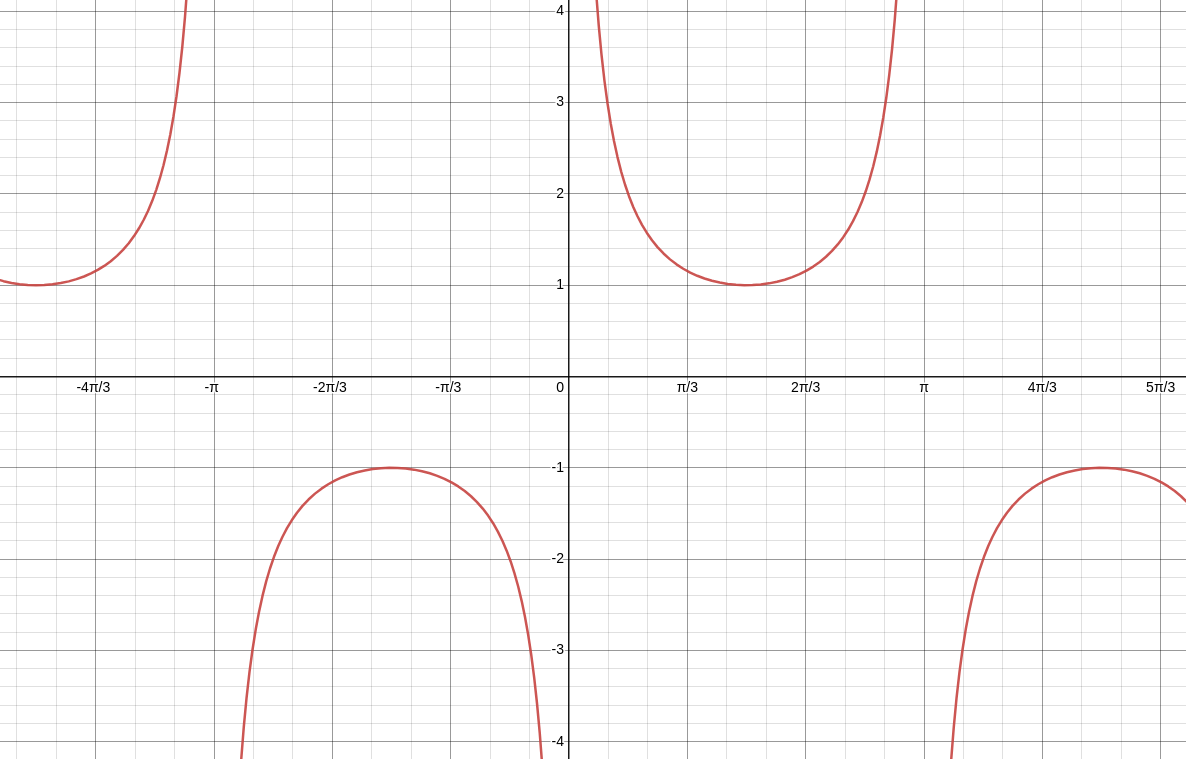
\includegraphics[scale=0.15]{images/csc.png} \\
    $\sec \theta = \dfrac{1}{\cos \theta}$        \\\\
    $\sec \theta = \dfrac{H}{A}$                  \\\\
    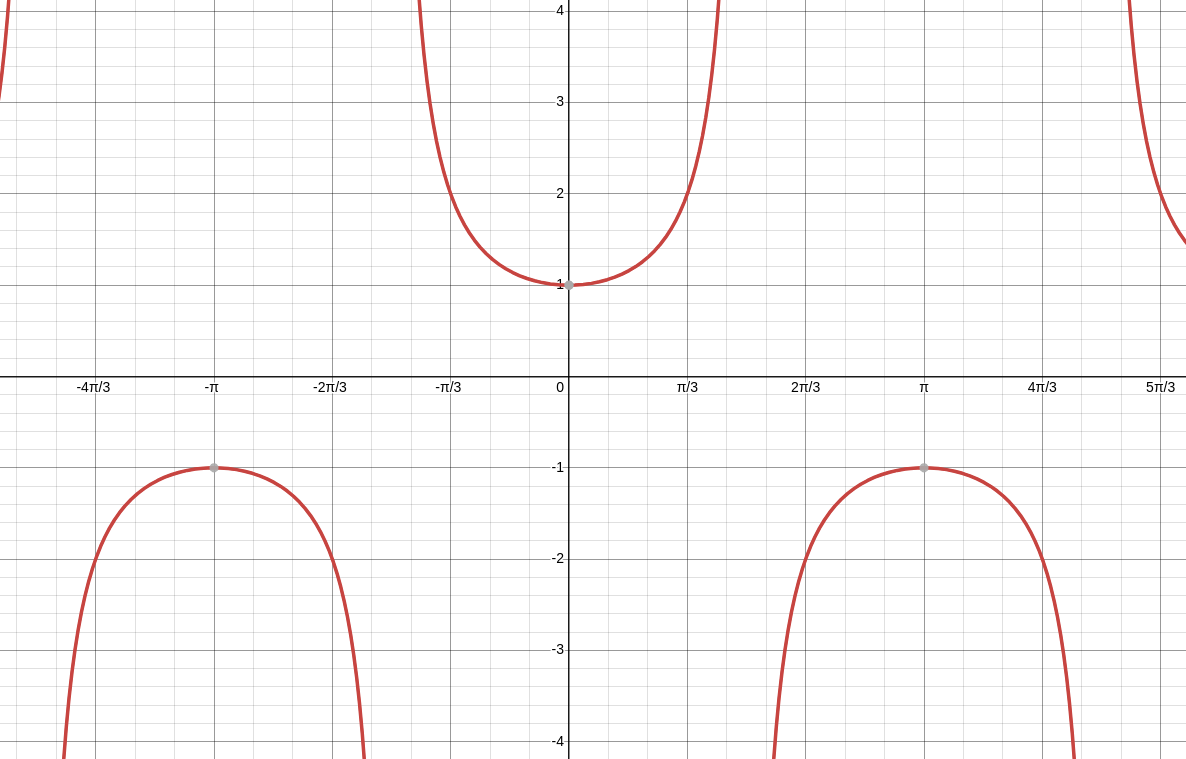
\includegraphics[scale=0.15]{images/sec.png} \\
    $\cot \theta = \dfrac{1}{\tan \theta} 
     = \dfrac{\cos \theta}{\sin \theta}$          \\\\
    $\cot \theta = \dfrac{A}{O}$                  \\\\
    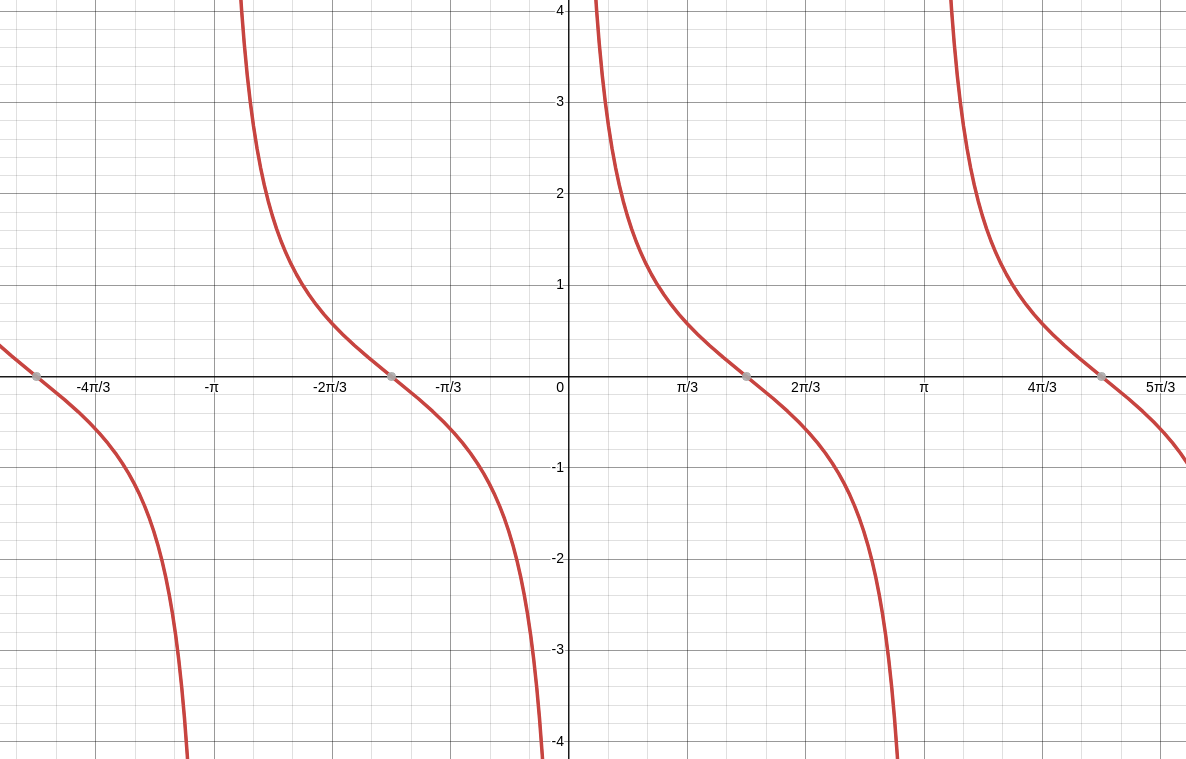
\includegraphics[scale=0.15]{images/cot.png} 
\end{multicols}
\hrule
\begin{multicols}{3}
    \noindent
    $\arcsin \theta = \sin^{-1} \theta$             \\\\
    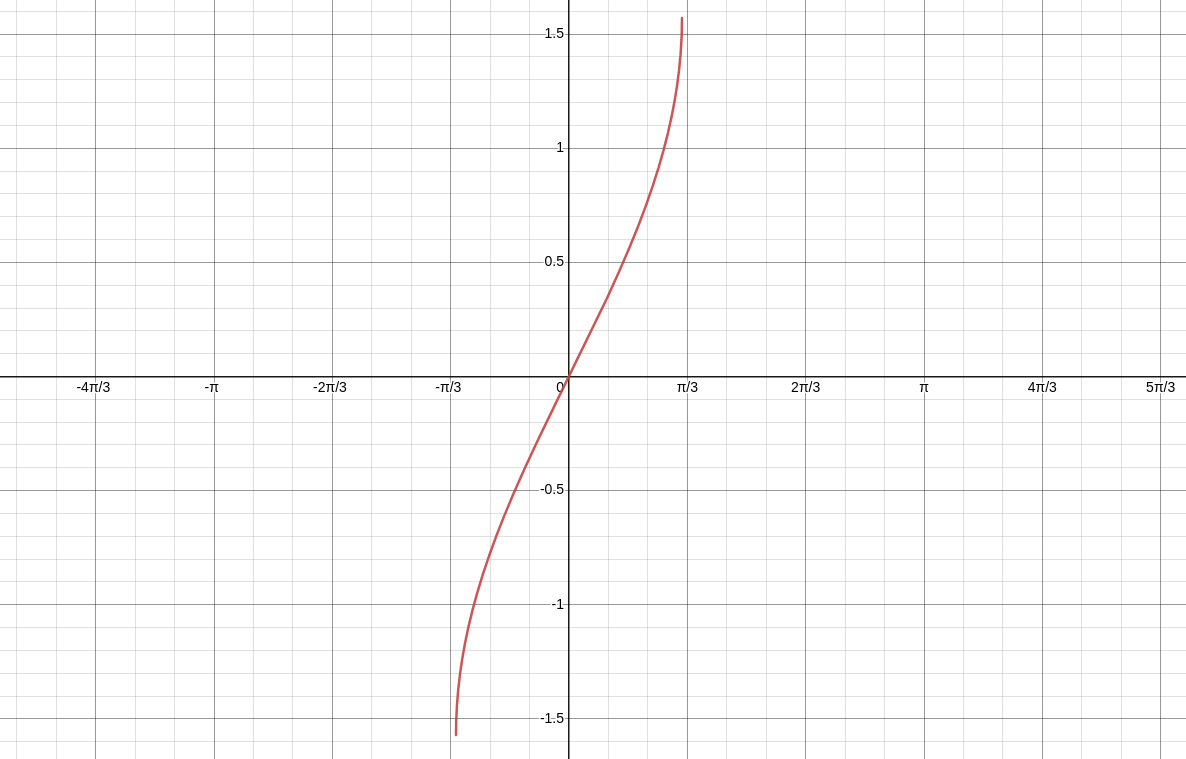
\includegraphics[scale=0.15]{images/arcsin.png} \\
    $\arccos \theta = \cos^{-1} \theta$             \\\\
    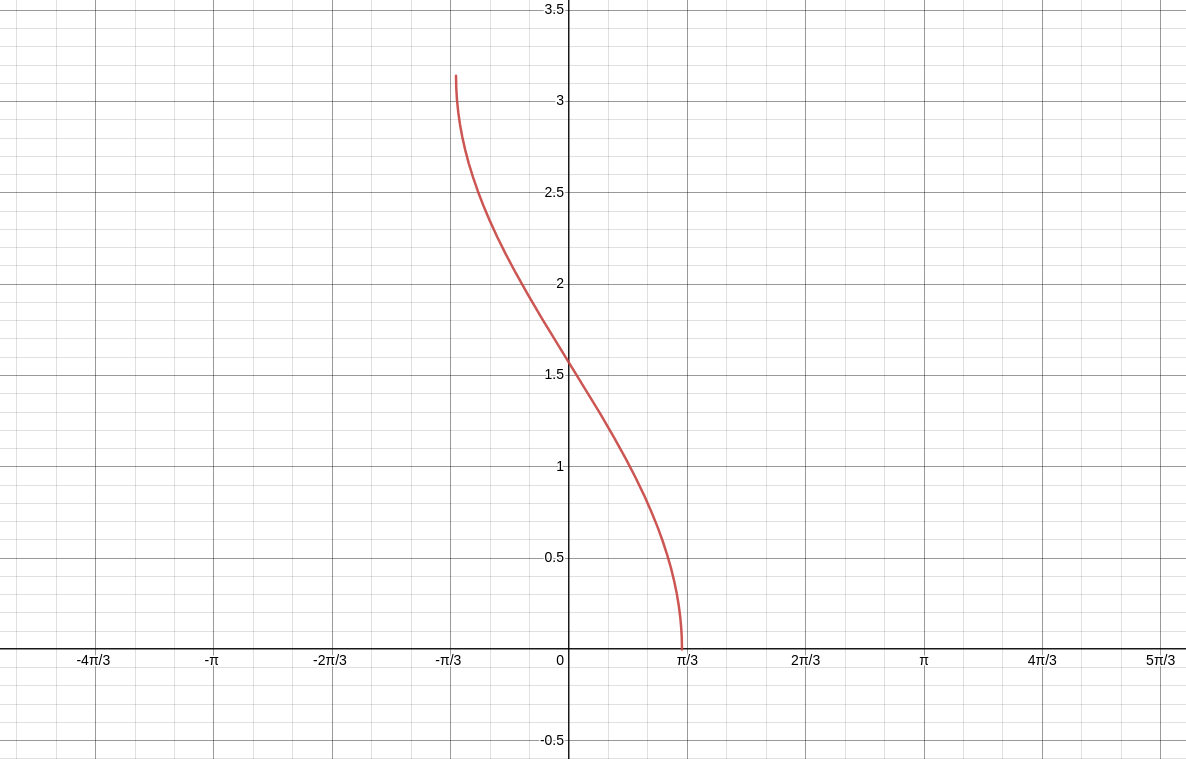
\includegraphics[scale=0.15]{images/arccos.png} \\
    $\arctan \theta = \tan^{-1} \theta$             \\\\
    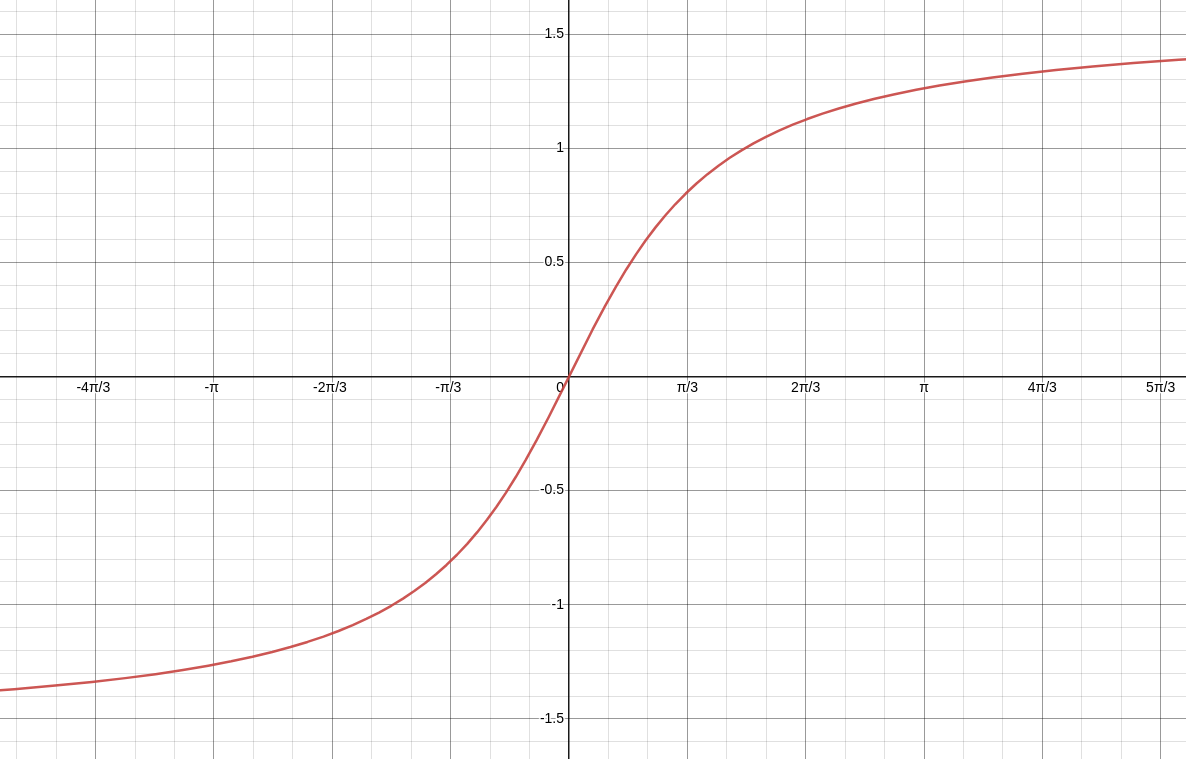
\includegraphics[scale=0.15]{images/arctan.png} 
\end{multicols}
\hrule
\end{document}